\scanpage{150}
\uline{Cylindre}\quad\deleted{\unsure{de}} $X$

trois ensembles à 2 éléments
\diagram{\[\begin{array}{ll|l}
a)&\pi_0\partial X&\varepsilon_0(X)\\
b)&\text{ens des deux générateurs de }\pi_1(X)\simeq H_1(X)&\varepsilon_1(X)\\
c)&\text{ens des deux orientations de }X&\omega(X)
\end{array}\]}
On a un iso. canonique
\[
\omega(X)\simeq\varepsilon_0(X)\wedge\varepsilon_1(X)
\]
Si on a une comp. \inserted{$S$} du bord ($\alpha\in\varepsilon_0(X)$) et une orientation du bord ($\beta\in\varepsilon_1(X)=\text{ens des deux génér. de }H_1(S)$) on a une orientation de $X$: celle qui induit $\beta$ sur $\alpha$ ...

\margin{\figure{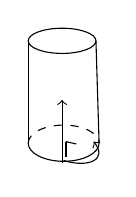
\begin{tikzpicture}[x=1cm,y=1cm]
\draw (0,0) ellipse (.43 and .16);
\draw (-.43,0)--(-.43,-1.3);\draw (.43,0)--(.47,-1.3);
\draw (-.43,-1.3) arc[start angle=180,end angle=360,x radius=.45,y radius=.23];
\draw[dashed] (-.43,-1.3) arc[start angle=180,end angle=0,x radius=.45,y radius=.23];
\draw[->] (0,-1.55)--(0,-.75);
\draw[->] (.02,-1.52) .. controls (.35,-1.62) and (.58,-1.5) .. (.4,-1.28);
\draw (.05,-1.28)--(.05,-1.48);\draw (.05,-1.28)--(.18,-1.31);
\end{tikzpicture}}}
Soit un autom \inserted{$u$} de $\unsure{\alpha|X}$ induisant l'identité sur $\partial X$. Il peut se relever en un autom. de $\widetilde X$ unique \inserted{$\widetilde u^{(S)}$} induisant l'identité sur $\widetilde X|S$ -- Alors son action sur $\widetilde X|S'$ est \deleted{\unsure{une}} \inserted{induite} par un élément \deleted{de} $n\in H_1(S')\xleftarrow{\sim}H_1(X)$. Si on \deleted{change} \inserted{remplace} $S$ par $S'$, on trouve $\widetilde u^{(S')}$, \deleted{\unsure{qui}}
\margin{$S'=\partial X\setminus S$}
\[
\widetilde u^{S'}=\tau_n^{-1}\widetilde u^S=\tau_{-n}\widetilde u^S
\]
\deleted{de} \unsure{qui|que} restreint à $S$ donne $\tau_{-n}$. Donc il y a un invariant qui est dans
\[
\begin{aligned}
H_1(X)\wedge_{\{\pm1\}}\varepsilon_0(X)
&=(\mathbb Z\wedge_{\pm1}\unsure{\varepsilon_0(X)|\varepsilon_1(X)})\wedge_{\pm1}\varepsilon_0(X)\\
&\simeq\mathbb Z\wedge_{\pm1}(\varepsilon_1(X)\wedge\varepsilon_0(X))\\
&\simeq\mathbb Z\wedge_{\pm1}\omega(X)
\end{aligned}
\]
\margin{150}
